\documentclass[12pt]{article}
\usepackage[top=1in,bottom=1in,left=1in,right=1in]{geometry}
\usepackage{alltt}
\usepackage{array}	
\usepackage{graphicx}
\usepackage{tabularx}
\usepackage{verbatim}
\usepackage{setspace}
\usepackage{listings}
\usepackage{amssymb,amsmath, amsthm}
\usepackage{qtree}
\usepackage{oz}
\usepackage[cc]{titlepic}
\usepackage{fancyvrb}
\usepackage{epstopdf}
\usepackage{soul}
\usepackage{array}
\usepackage{tikz}
\usepackage{float}
\usepackage{booktabs}
\usepackage[
    pdfborder={0 0 0},
]{hyperref}
%\usepackage{tabulary}
\usetikzlibrary{matrix}
\usetikzlibrary{fit}
%\newcolumntype{L}{>{\centering\arraybackslash}m{3cm}}

\title{Concordia University\\
Department of Computer Science and Software Engineering\\
\textbf{SOEN 331 - S and U\\Introduction to Formal Methods\\for Software Engineering}\\
\ \\
\textbf{Assignment 4 - Solutions}\\
Temporal Logic\\
\textbf{Team 19 - Section U}}
\author{
	\textbf{Samuel Boaknin}\\
	\texttt{40009692}
	\and
	\textbf{Ryan Leyland}\\
	\texttt{40015165}
	\and
	\textbf{Saleha Tariq}\\
	\texttt{40006997}
	\and
	\textbf{Meng Susana Ung}\\
	\texttt{40099729}
}
\date{Date: April 19, 2021}

\begin{document}
\maketitle

\newpage
\tableofcontents
\newpage

\section{Question 1}
\renewcommand\labelenumi{(\theenumi)}
\begin{enumerate}


\item %\leavevmode\vadjust{\vspace{-\baselineskip}}\newline

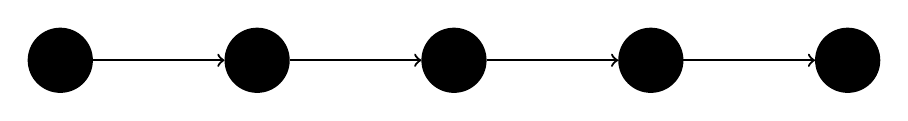
\begin{tikzpicture}[baseline=(current  bounding  box.center), thick]
\node [circle, draw, fill=black, minimum size=.8cm] (a1) at (0,0) {};
\node [circle, draw, fill=black, minimum size=.8cm] (a2) at (2.5,0) {};
\node [circle, draw, fill=black, minimum size=.8cm] (a3) at (5,0) {};
\node [circle, draw, fill=black, minimum size=.8cm] (a4) at (7.5,0) {};
\node [circle, draw, fill=black, minimum size=.8cm] (a5) at (10,0) {};

\draw[->] (a1) -- (a2); 
\draw[->] (a2) -- (a3);
\draw[->] (a3) -- (a4);
\draw[->] (a4) -- (a5);
\end{tikzpicture}
\begin{table}[H]
%\centering
\hspace{1cm}\begin{tabular}{p{0.72cm}p{1cm}p{0.72cm}p{1cm}p{0.72cm}p{1cm}p{0.72cm}p{1cm}p{0.72cm}p{1cm}p{0.72cm}p{1cm}}
a & & e & & e & & e & &  g \\
c \\
e \\
\end{tabular}
%\caption{}
\label{tab:Q1_1}
\end{table}


\item 
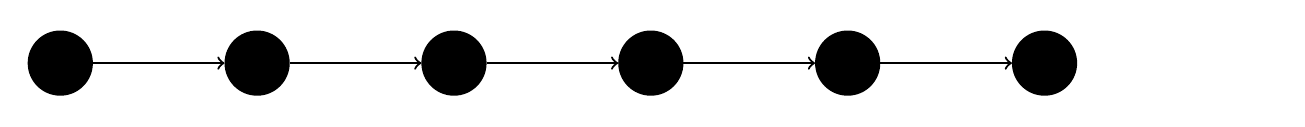
\begin{tikzpicture}[baseline=(current  bounding  box.center), thick]
\node [circle, draw, fill=black, minimum size=.8cm] (a1) at (0,0) {};
\node [circle, draw, fill=black, minimum size=.8cm] (a2) at (2.5,0) {};
\node [circle, draw, fill=black, minimum size=.8cm] (a3) at (5,0) {};
\node [circle, draw, fill=black, minimum size=.8cm] (a4) at (7.5,0) {};
\node [circle, draw, fill=black, minimum size=.8cm] (a5) at (10,0) {};
\node [circle, draw, fill=black, minimum size=.8cm] (a6) at (12.5,0) {};
\node [circle, minimum size=.9cm] (a7) at (15,0) {};

\draw[->] (a1) -- (a2); 
\draw[->] (a2) -- (a3);
\draw[->] (a3) -- (a4);
\draw[->] (a4) -- (a5);
\draw[->] (a5) -- (a6);
\end{tikzpicture}
\begin{table}[H]
%\centering
\hspace{1cm}\begin{tabular}{p{0.72cm}p{1cm}p{0.72cm}p{1cm}p{0.72cm}p{1cm}p{0.72cm}p{1cm}p{0.72cm}p{0.8cm}p{0.72cm}p{1cm}}
a & & y & & y & & y & & x & & w \\
d & & & & & & & & y \\
\end{tabular}
%\caption{}
\label{tab:Q1_2}
\end{table}


\item 
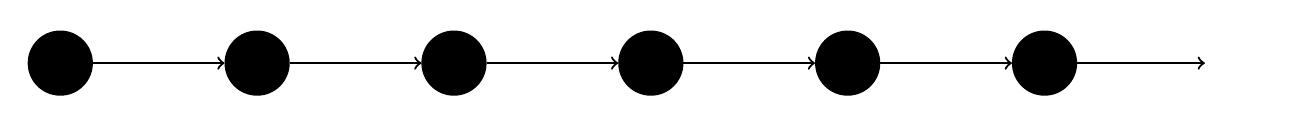
\begin{tikzpicture}[baseline=(current  bounding  box.center), thick]
\node [circle, draw, fill=black, minimum size=.8cm] (a1) at (0,0) {};
\node [circle, draw, fill=black, minimum size=.8cm] (a2) at (2.5,0) {};
\node [circle, draw, fill=black, minimum size=.8cm] (a3) at (5,0) {};
\node [circle, draw, fill=black, minimum size=.8cm] (a4) at (7.5,0) {};
\node [circle, draw, fill=black, minimum size=.8cm] (a5) at (10,0) {};
\node [circle, draw, fill=black, minimum size=.8cm] (a6) at (12.5,0) {};
\node [circle, minimum size=.9cm] (a7) at (15,0) {};

\draw[->] (a1) -- (a2); 
\draw[->] (a2) -- (a3);
\draw[->] (a3) -- (a4);
\draw[->] (a4) -- (a5);
\draw[->] (a5) -- (a6);
\draw[->] (a6) -- (a7);
\end{tikzpicture}
\begin{table}[H]
%\centering
\hspace{1cm}\begin{tabular}{p{0.72cm}p{1cm}p{0.72cm}p{1cm}p{0.72cm}p{1cm}p{0.72cm}p{1cm}p{0.72cm}p{0.8cm}p{0.72cm}p{1cm}}
a & & y & & y & & y & & x & & z \\
d & & & & & & & & y & & n \\
\end{tabular}
%\caption{}
\label{tab:Q1_3}
\end{table}

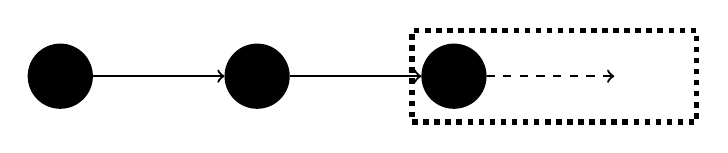
\begin{tikzpicture}[baseline=(current  bounding  box.center), thick]
\node [circle, draw, fill=black, minimum size=.8cm] (a1) at (0,0) {};
\node [circle, draw, fill=black, minimum size=.8cm] (a2) at (2.5,0) {};
\node [circle, draw, fill=black, minimum size=.8cm] (a3) at (5,0) {};
\node [circle, minimum size=.9cm] (a4) at (7.5,0) {};
\node [fit=(a3) (a4),line width=2pt,draw,dotted,black] {};

\draw[->] (a1) -- (a2); 
\draw[->] (a2) -- (a3);
\draw[dashed, ->] (a3) -- (a4);
\end{tikzpicture}
\begin{table}[H]
%\centering
\hspace{1cm}\begin{tabular}{p{0.72cm}p{1cm}p{0.72cm}p{1cm}p{0.72cm}p{1cm}p{0.72cm}p{1cm}p{0.72cm}p{0.8cm}p{0.72cm}p{1cm}}
b & & y & & y ... \\
d & \\
\end{tabular}
%\caption{}
\label{tab:Q1_3cont}
\end{table}


\item 
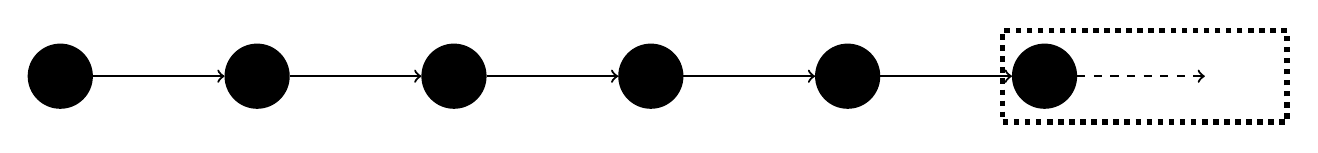
\begin{tikzpicture}[baseline=(current  bounding  box.center), thick]
\node [circle, draw, fill=black, minimum size=.8cm] (a1) at (0,0) {};
\node [circle, draw, fill=black, minimum size=.8cm] (a2) at (2.5,0) {};
\node [circle, draw, fill=black, minimum size=.8cm] (a3) at (5,0) {};
\node [circle, draw, fill=black, minimum size=.8cm] (a4) at (7.5,0) {};
\node [circle, draw, fill=black, minimum size=.8cm] (a5) at (10,0) {};
\node [circle, draw, fill=black, minimum size=.8cm] (a6) at (12.5,0) {};
\node [circle, minimum size=.9cm] (a7) at (15,0) {};
\node [fit=(a6) (a7),line width=2pt,draw,dotted,black] {};

\draw[->] (a1) -- (a2); 
\draw[->] (a2) -- (a3);
\draw[->] (a3) -- (a4);
\draw[->] (a4) -- (a5);
\draw[->] (a5) -- (a6);
\draw[dashed, ->] (a6) -- (a7);
\end{tikzpicture}
\begin{table}[H]
%\centering
\hspace{1cm}\begin{tabular}{p{0.72cm}p{1cm}p{0.72cm}p{1cm}p{0.72cm}p{1cm}p{0.72cm}p{1cm}p{0.72cm}p{0.8cm}p{0.72cm}p{1cm}}
b & & y & & y & & y & & y & & y ... \\
c & & & & & & & & g \\
\end{tabular}
%\caption{}
\label{tab:Q1_4}
\end{table}


\item 
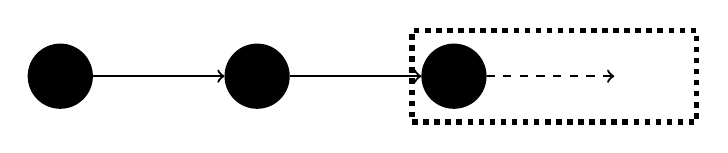
\begin{tikzpicture}[baseline=(current  bounding  box.center), thick]
\node [circle, draw, fill=black, minimum size=.8cm] (a1) at (0,0) {};
\node [circle, draw, fill=black, minimum size=.8cm] (a2) at (2.5,0) {};
\node [circle, draw, fill=black, minimum size=.8cm] (a3) at (5,0) {};4
\node [circle, minimum size=.9cm] (a4) at (7.5,0) {};

\draw[->] (a1) -- (a2); 
\draw[->] (a2) -- (a3);
\draw[dashed, ->] (a3) -- (a4);
\node [fit=(a3) (a4),line width=2pt,draw,dotted,black] {};

\end{tikzpicture}
\begin{table}[H]
%\centering
\hspace{1cm}\begin{tabular}{p{0.72cm}p{1cm}p{0.72cm}p{1cm}p{0.72cm}p{1cm}p{0.72cm}p{1cm}p{0.72cm}p{0.8cm}p{0.72cm}p{1cm}}
b & & y & & y ... \\
d  \\
\end{tabular}
%\caption{}
\label{tab:Q1_5}
\end{table}



\item 
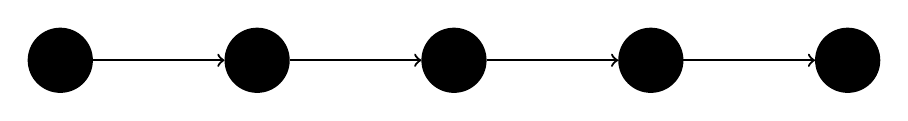
\begin{tikzpicture}[baseline=(current  bounding  box.center), thick]
\node [circle, draw, fill=black, minimum size=.8cm] (a1) at (0,0) {};
\node [circle, draw, fill=black, minimum size=.8cm] (a2) at (2.5,0) {};
\node [circle, draw, fill=black, minimum size=.8cm] (a3) at (5,0) {};
\node [circle, draw, fill=black, minimum size=.8cm] (a4) at (7.5,0) {};
\node [circle, draw, fill=black, minimum size=.8cm] (a5) at (10,0) {};

\draw[->] (a1) -- (a2); 
\draw[->] (a2) -- (a3);
\draw[->] (a3) -- (a4);
\draw[->] (a4) -- (a5);
\end{tikzpicture}
\begin{table}[H]
%\centering
\hspace{1cm}\begin{tabular}{p{0.72cm}p{1cm}p{0.72cm}p{1cm}p{0.72cm}p{1cm}p{0.72cm}p{1cm}p{0.72cm}p{0.8cm}p{0.72cm}p{1cm}}
c & & & & & & & & g \\
\end{tabular}
%\caption{}
\label{tab:Q1_6}
\end{table}


\item 
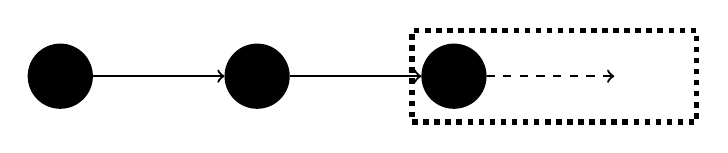
\begin{tikzpicture}[baseline=(current  bounding  box.center), thick]
\node [circle, draw, fill=black, minimum size=.8cm] (a1) at (0,0) {};
\node [circle, draw, fill=black, minimum size=.8cm] (a2) at (2.5,0) {};
\node [circle, draw, fill=black, minimum size=.8cm] (a3) at (5,0) {};
\node [circle, minimum size=.9cm] (a4) at (7.5,0) {};
\node [fit=(a3) (a4),line width=2pt,draw,dotted,black] {};

\draw[->] (a1) -- (a2); 
\draw[->] (a2) -- (a3);
\draw[dashed, ->] (a3) -- (a4);
\end{tikzpicture}
\begin{table}[H]
%\centering
\hspace{1cm}\begin{tabular}{p{0.72cm}p{1cm}p{0.72cm}p{1cm}p{0.72cm}p{1cm}p{0.72cm}p{1cm}p{0.72cm}p{0.8cm}p{0.72cm}p{1cm}}
d & & y & & y ... \\
\end{tabular}
%\caption{}
\label{tab:Q1_7}
\end{table}

There exists three model's whereby the program terminates, given by the following expressions: \\
$<(a \land c \land e),~e,~e,~e,~g>$ \\ 
$<(a \land d),~y,~y,~y,~(x \land y),~w>$ \\
$<c,~\emptyset,~\emptyset,~\emptyset,~g>$ \\

\end{enumerate}



\newpage
\section{Question 2}
\renewcommand\labelenumi{(\theenumi)}
\begin{enumerate}

\item %\leavevmode\vadjust{\vspace{-\baselineskip}}\newline
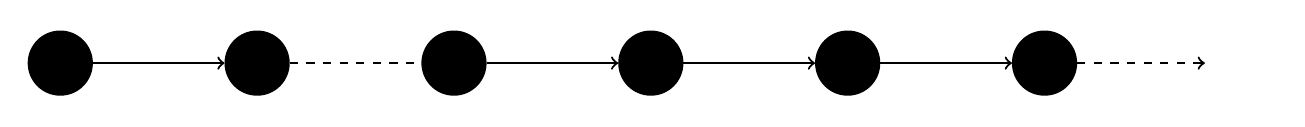
\begin{tikzpicture}[baseline=(current  bounding  box.center), thick]
\node [circle, draw, fill=black, minimum size=.8cm] (a1) at (0,0) {};
\node [circle, draw, fill=black, minimum size=.8cm] (a2) at (2.5,0) {};
\node [circle, draw, fill=black, minimum size=.8cm] (a3) at (5,0) {};
\node [circle, draw, fill=black, minimum size=.8cm] (a4) at (7.5,0) {};
\node [circle, draw, fill=black, minimum size=.8cm] (a5) at (10,0) {};
\node [circle, draw, fill=black, minimum size=.8cm] (a6) at (12.5,0) {};
\node [circle, minimum size=.9cm] (a7) at (15,0) {};

\draw[->] (a1) -- (a2); 
\draw[dashed] (a2) -- (a3);
\draw[->] (a3) -- (a4);
\draw[->] (a4) -- (a5);
\draw[->] (a5) -- (a6);
\draw[dashed, ->] (a6) -- (a7);
\end{tikzpicture}
\begin{table}[H]
%\centering
\hspace{1cm}\begin{tabular}{p{0.72cm}p{0.9cm}p{0.72cm}p{0.9cm}p{0.72cm}p{0.9cm}p{0.72cm}p{0.9cm}p{0.72cm}p{0.9cm}p{0.72cm}p{0.9cm}}
$\phi$ &  &$\phi$ & ... &  &  &  &  &  &  &  &  \\
$\psi$ &  &  &  &  &  &  &  &  &  &  &  \\
  &\textbf{or} & $\psi$ &  &  &  &  &  &  &  &  &  \\
  &  &  & \textbf{or} & $\psi$ &  &  &  &  &  &  & 
\end{tabular}
%\caption{}
\label{tab:Q2_1}
\end{table}
If $\phi$ is an invariant, then $\psi$ is true in some moment in time.\\

\item 
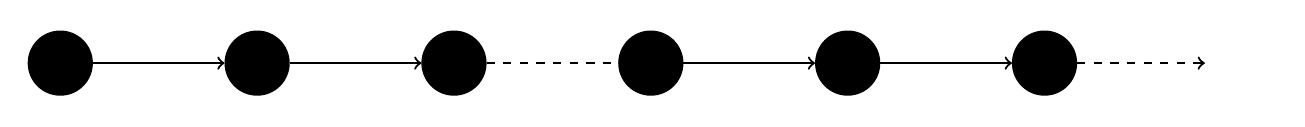
\begin{tikzpicture}[baseline=(current  bounding  box.center), thick]
\node [circle, draw, fill=black, minimum size=.8cm] (a1) at (0,0) {};
\node [circle, draw, fill=black, minimum size=.8cm] (a2) at (2.5,0) {};
\node [circle, draw, fill=black, minimum size=.8cm] (a3) at (5,0) {};
\node [circle, draw, fill=black, minimum size=.8cm] (a4) at (7.5,0) {};
\node [circle, draw, fill=black, minimum size=.8cm] (a5) at (10,0) {};
\node [circle, draw, fill=black, minimum size=.8cm] (a6) at (12.5,0) {};
\node [circle, minimum size=.9cm] (a7) at (15,0) {};

\draw[->] (a1) -- (a2); 
\draw[->] (a2) -- (a3);
\draw[dashed] (a3) -- (a4);
\draw[->] (a4) -- (a5);
\draw[->] (a5) -- (a6);
\draw[dashed, ->] (a6) -- (a7);
\end{tikzpicture}
\begin{table}[H]
%\centering
\hspace{1cm}\begin{tabular}{p{0.72cm}p{0.9cm}p{0.72cm}p{0.9cm}p{0.72cm}p{0.9cm}p{0.72cm}p{0.9cm}p{0.72cm}p{0.9cm}p{0.72cm}p{0.9cm}}
$\phi$ &  & $\phi$ &  & $\phi$ & ... &  &  &  &  &  &  \\
 &  & $\psi$ &  & $\psi$ & ... &  &  &  &  &  &  \\
 &  &  & \textbf{or} & $\psi$ &  & $\psi$ & ... &  &  &  &  \\
 &  &  &  &  & \textbf{or} & $\psi$ &  & $\psi$ & ... &  & 
\end{tabular}
%\caption{}
\label{tab:Q2_2}
\end{table}
If $\phi$ is an invariant, then from $i+1$ onwards, $\psi$ will always eventually become true.\\

\item %\leavevmode\vadjust{\vspace{-\baselineskip}}\newline
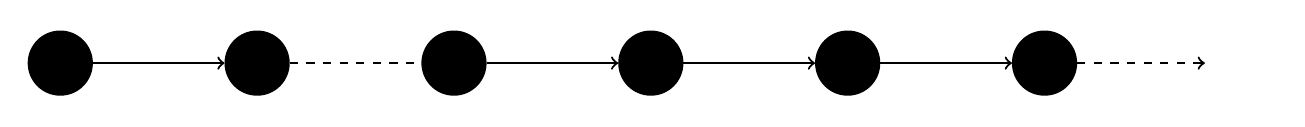
\begin{tikzpicture}[baseline=(current  bounding  box.center), thick]
\node [circle, draw, fill=black, minimum size=.8cm] (a1) at (0,0) {};
\node [circle, draw, fill=black, minimum size=.8cm] (a2) at (2.5,0) {};
\node [circle, draw, fill=black, minimum size=.8cm] (a3) at (5,0) {};
\node [circle, draw, fill=black, minimum size=.8cm] (a4) at (7.5,0) {};
\node [circle, draw, fill=black, minimum size=.8cm] (a5) at (10,0) {};
\node [circle, draw, fill=black, minimum size=.8cm] (a6) at (12.5,0) {};
\node [circle, minimum size=.9cm] (a7) at (15,0) {};

\draw[->] (a1) -- (a2); 
\draw[dashed] (a2) -- (a3);
\draw[->] (a3) -- (a4);
\draw[->] (a4) -- (a5);
\draw[->] (a5) -- (a6);
\draw[dashed, ->] (a6) -- (a7);
\end{tikzpicture}
\begin{table}[H]
%\centering
\hspace{1cm}\begin{tabular}{p{0.72cm}p{0.9cm}p{0.72cm}p{0.9cm}p{0.72cm}p{0.9cm}p{0.72cm}p{0.9cm}p{0.72cm}p{0.9cm}p{0.72cm}p{0.9cm}}
$\phi$ &  & $\psi$ &  &  &  &  &  &  &  &  &  \\
$\tau$ &  & $\tau$ & ... &  &  &  &  &  &  &  &  \\
 & \textbf{or} & $\tau$ & \textbf{} & $\tau$ & ... &  &  &  &  &  &  \\
 &  &  & \textbf{or} & $\tau$ & \textbf{} & $\tau$ & ... &  &  &  & 
\end{tabular}
%\caption{}
\label{tab:Q2_3}
\end{table}
If $\phi$ is true at $i$ and $\psi$ is true at $i+1$, then $\tau$ can become an invariant anywhere on the path.\\

\item %\leavevmode\vadjust{\vspace{-\baselineskip}}\newline
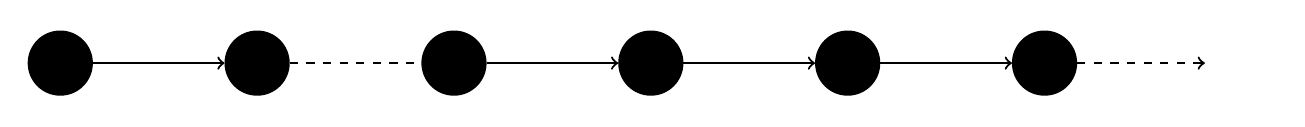
\begin{tikzpicture}[baseline=(current  bounding  box.center), thick]
\node [circle, draw, fill=black, minimum size=.8cm] (a1) at (0,0) {};
\node [circle, draw, fill=black, minimum size=.8cm] (a2) at (2.5,0) {};
\node [circle, draw, fill=black, minimum size=.8cm] (a3) at (5,0) {};
\node [circle, draw, fill=black, minimum size=.8cm] (a4) at (7.5,0) {};
\node [circle, draw, fill=black, minimum size=.8cm] (a5) at (10,0) {};
\node [circle, draw, fill=black, minimum size=.8cm] (a6) at (12.5,0) {};
\node [circle, minimum size=.9cm] (a7) at (15,0) {};

\draw[->] (a1) -- (a2); 
\draw[dashed] (a2) -- (a3);
\draw[->] (a3) -- (a4);
\draw[->] (a4) -- (a5);
\draw[->] (a5) -- (a6);
\draw[dashed, ->] (a6) -- (a7);
\end{tikzpicture}
\begin{table}[H]
%\centering
\hspace{1cm}\begin{tabular}{p{0.72cm}p{0.9cm}p{0.72cm}p{0.9cm}p{0.72cm}p{0.9cm}p{0.72cm}p{0.9cm}p{0.72cm}p{0.9cm}p{0.72cm}p{0.9cm}}
$\psi$ &  & $\chi$ &  &  &  &  &  &  &  &  &  \\
 &  & $\tau$ &  &  &  &  &  &  &  &  &
\end{tabular}
%\caption{}
\label{tab:Q2_4}
\end{table}
If $\psi$ is true at $i$ and $\chi$ is true at $i+1$, then $\tau$ is also true at $i+1$.\\

\item 
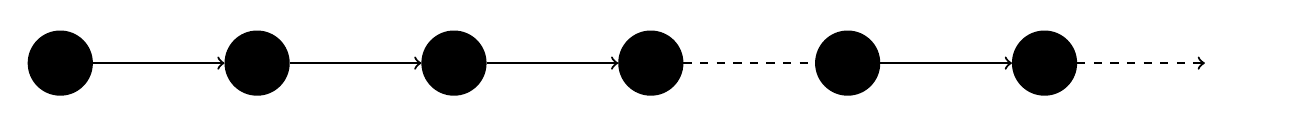
\begin{tikzpicture}[baseline=(current  bounding  box.center), thick]
\node [circle, draw, fill=black, minimum size=.8cm] (a1) at (0,0) {};
\node [circle, draw, fill=black, minimum size=.8cm] (a2) at (2.5,0) {};
\node [circle, draw, fill=black, minimum size=.8cm] (a3) at (5,0) {};
\node [circle, draw, fill=black, minimum size=.8cm] (a4) at (7.5,0) {};
\node [circle, draw, fill=black, minimum size=.8cm] (a5) at (10,0) {};
\node [circle, draw, fill=black, minimum size=.8cm] (a6) at (12.5,0) {};
\node [circle, minimum size=.9cm] (a7) at (15,0) {};

\draw[->] (a1) -- (a2); 
\draw[->] (a2) -- (a3);
\draw[->] (a3) -- (a4);
\draw[dashed] (a4) -- (a5);
\draw[->] (a5) -- (a6);
\draw[dashed, ->] (a6) -- (a7);
\end{tikzpicture}
\begin{table}[H]
%\centering
\hspace{1cm}\begin{tabular}{p{0.72cm}p{0.9cm}p{0.72cm}p{0.9cm}p{0.72cm}p{0.9cm}p{0.72cm}p{0.9cm}p{0.72cm}p{0.9cm}p{0.72cm}p{0.9cm}}
$\chi$ &  & $\omega$ &  & $\phi$ &  & $\phi$ &  & $\psi$ &  &  &  \\
 &  &  &  &  &  &  &  & \texttildelow $\phi$ &  &  & 
\end{tabular}
%\caption{}
\label{tab:Q2_5}
\end{table}
If $\chi$ is true at $i$ and $\omega$ is true at $i+1$, then from $i+2$ onwards, $\phi$ is true until $\psi$ becomes true.\\

\item
%\leavevmode\vadjust{\vspace{-\baselineskip}}\newline
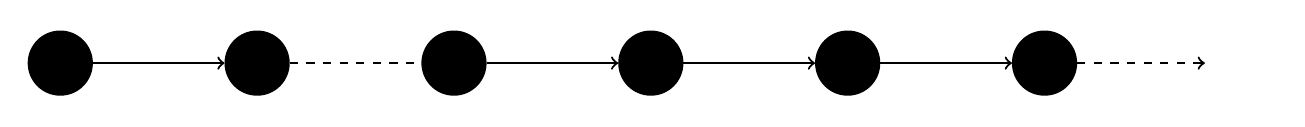
\begin{tikzpicture}[baseline=(current  bounding  box.center), thick]
\node [circle, draw, fill=black, minimum size=.8cm] (a1) at (0,0) {};
\node [circle, draw, fill=black, minimum size=.8cm] (a2) at (2.5,0) {};
\node [circle, draw, fill=black, minimum size=.8cm] (a3) at (5,0) {};
\node [circle, draw, fill=black, minimum size=.8cm] (a4) at (7.5,0) {};
\node [circle, draw, fill=black, minimum size=.8cm] (a5) at (10,0) {};
\node [circle, draw, fill=black, minimum size=.8cm] (a6) at (12.5,0) {};
\node [circle, minimum size=.9cm] (a7) at (15,0) {};

\draw[->] (a1) -- (a2); 
\draw[dashed] (a2) -- (a3);
\draw[->] (a3) -- (a4);
\draw[->] (a4) -- (a5);
\draw[->] (a5) -- (a6);
\draw[dashed, ->] (a6) -- (a7);
\end{tikzpicture}
\begin{table}[H]
%\centering
\hspace{1cm}\begin{tabular}{p{0.72cm}p{0.9cm}p{0.72cm}p{0.9cm}p{0.72cm}p{0.9cm}p{0.72cm}p{0.9cm}p{0.72cm}p{0.9cm}p{0.72cm}p{0.9cm}}
$\phi$ &  &  & ... &  &  &  &  &  &  &  &  \\
$\omega$ & & $\omega$ & & $\omega$ & & $\omega$ & & $\omega$ & & $\omega$ &  \\
\end{tabular}
%\caption{}
\label{tab:Q2_6}
\end{table}
%\leavevmode\vadjust{\vspace{-\baselineskip}}\newline
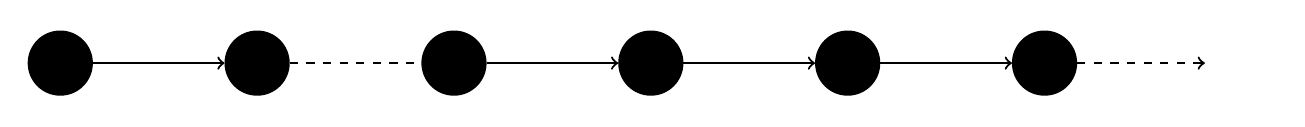
\begin{tikzpicture}[baseline=(current  bounding  box.center), thick]
\node [circle, draw, fill=black, minimum size=.8cm] (a1) at (0,0) {};
\node [circle, draw, fill=black, minimum size=.8cm] (a2) at (2.5,0) {};
\node [circle, draw, fill=black, minimum size=.8cm] (a3) at (5,0) {};
\node [circle, draw, fill=black, minimum size=.8cm] (a4) at (7.5,0) {};
\node [circle, draw, fill=black, minimum size=.8cm] (a5) at (10,0) {};
\node [circle, draw, fill=black, minimum size=.8cm] (a6) at (12.5,0) {};
\node [circle, minimum size=.9cm] (a7) at (15,0) {};

\draw[->] (a1) -- (a2); 
\draw[dashed] (a2) -- (a3);
\draw[->] (a3) -- (a4);
\draw[->] (a4) -- (a5);
\draw[->] (a5) -- (a6);
\draw[dashed, ->] (a6) -- (a7);
\end{tikzpicture}
\begin{table}[H]
%\centering
\hspace{1cm}\begin{tabular}{p{0.72cm}p{0.9cm}p{0.72cm}p{0.9cm}p{0.72cm}p{0.9cm}p{0.72cm}p{0.9cm}p{0.72cm}p{0.9cm}p{0.72cm}p{0.9cm}}
$\psi$ &  & & ... &  &  &  &  &  &  &  &  \\
$\omega$ & & $\omega$ & & $\omega$ & & $\omega$ & & $\omega$ & & $\omega$ &  \\
\end{tabular}
%\caption{}
\end{table}

If only one of the mutually exclusive events $\phi$ or $\psi$ is true, then  $\omega$ will always be true.\\
\item
%\leavevmode\vadjust{\vspace{-\baselineskip}}\newline
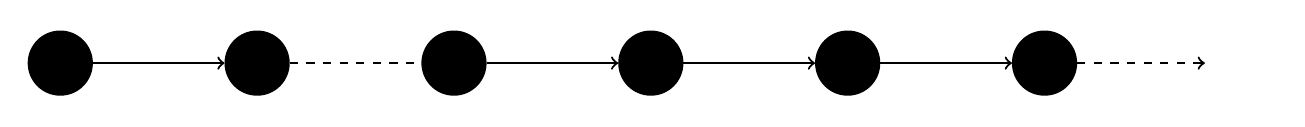
\begin{tikzpicture}[baseline=(current  bounding  box.center), thick]
\node [circle, draw, fill=black, minimum size=.8cm] (a1) at (0,0) {};
\node [circle, draw, fill=black, minimum size=.8cm] (a2) at (2.5,0) {};
\node [circle, draw, fill=black, minimum size=.8cm] (a3) at (5,0) {};
\node [circle, draw, fill=black, minimum size=.8cm] (a4) at (7.5,0) {};
\node [circle, draw, fill=black, minimum size=.8cm] (a5) at (10,0) {};
\node [circle, draw, fill=black, minimum size=.8cm] (a6) at (12.5,0) {};
\node [circle, minimum size=.9cm] (a7) at (15,0) {};

\draw[->] (a1) -- (a2); 
\draw[dashed] (a2) -- (a3);
\draw[->] (a3) -- (a4);
\draw[->] (a4) -- (a5);
\draw[->] (a5) -- (a6);
\draw[dashed, ->] (a6) -- (a7);
\end{tikzpicture}
\begin{table}[H]
%\centering
\hspace{1cm}\begin{tabular}{p{0.72cm}p{0.9cm}p{0.72cm}p{0.9cm}p{0.72cm}p{0.9cm}p{0.72cm}p{0.9cm}p{0.72cm}p{0.9cm}p{0.72cm}p{0.9cm}}
$\chi$  &  & $\chi$ &     &  &  &  &  &  &  &  &  \\
        &  & $\psi$ & &  &  &  &  &  &  &  &  \\
$\omega$&    &  &   &  &  &  &  &  &  \\
        & or & $\omega$ &   & & &  &  &  &  \\
        &  & &  or & $\omega$ & ... &  &  &  &  \\
\end{tabular}
%\caption{}
\label{tab:Q2_7}
\end{table}
If $\chi$ is true at $i$ and $\chi$ \& $\psi$ is true at $i+1$, then $\omega$ can emerge anywhere on the path.\\
\newpage
\item
%\leavevmode\vadjust{\vspace{-\baselineskip}}\newline
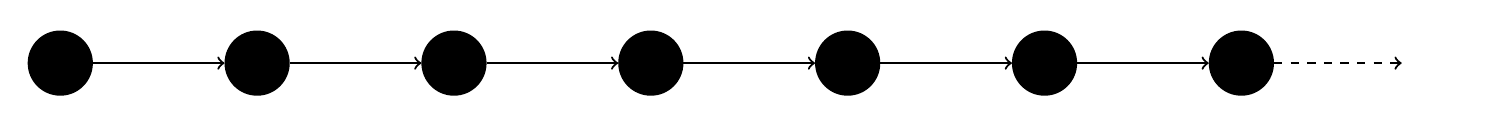
\begin{tikzpicture}[baseline=(current  bounding  box.center), thick]
\node [circle, draw, fill=black, minimum size=.8cm] (a1) at (0,0) {};
\node [circle, draw, fill=black, minimum size=.8cm] (a2) at (2.5,0) {};
\node [circle, draw, fill=black, minimum size=.8cm] (a3) at (5,0) {};
\node [circle, draw, fill=black, minimum size=.8cm] (a4) at (7.5,0) {};
\node [circle, draw, fill=black, minimum size=.8cm] (a5) at (10,0) {};
\node [circle, draw, fill=black, minimum size=.8cm] (a6) at (12.5,0) {};
\node [circle, draw, fill=black, minimum size=.8cm] (a7) at (15,0) {};\
\node [circle, minimum size=.9cm] (a8) at (17.5,0) {};\

\draw[->] (a1) -- (a2); 
\draw[->] (a2) -- (a3);
\draw[->] (a3) -- (a4);
\draw[->] (a4) -- (a5);
\draw[->] (a5) -- (a6);
\draw[->] (a6) -- (a7);
\draw[dashed, ->] (a7) -- (a8);
\end{tikzpicture}
\begin{table}[H]
%\centering
\hspace{1cm}\begin{tabular}{p{0.72cm}p{0.9cm}p{0.72cm}p{0.9cm}p{0.72cm}p{0.9cm}p{0.72cm}p{0.9cm}p{0.72cm}p{0.9cm}p{0.72cm}p{0.9cm}}
$\chi$ & &  & & $\psi$ & &        & &        & &  &  \\
$\mu $ & &  & & $\tau$ & & $\tau$ & & $\tau$ & & $\omega$ &  \\
&  &  &  &  &  &  &  & & & \texttildelow $\tau$ &
\end{tabular}
\label{tab:Q2_8}
%\caption{}
\end{table}

If $\chi$ is true at $i$ and $\psi$ is true at $i+2$, then from $i+2$ onwards, $\tau$ is true unless $\omega$ becomes true. If $\mu$ is true at $i$, then $\omega$ will be true at $i+5$.\\
\end{enumerate}
\end{document}